\section{Theory}\label{sec:theory}

In this section, we will discuss the theoretical foundations of message passing neural networks (MPNNs) and ensembles for predicting
the binding energy of molecules in a catalyst process.

\subsection{Message Passing Neural Networks}\label{subsec:modelling_task}

The key idea behind MPNNs is the concept of
message passing, where each node in the graph exchanges information with its neighbors in an iterative manner.

Let $G = (N, E)$ be a graph, where $N$ is the set of nodes and $E$ is the set of edges.
Each node $n \in N$ is associated with an invariant representation vector $\mathbf{S}_{n} \in \mathbb{R}^{Fx1}$,
an equivariant representation
vector $\vec{\mathbf{v}}_{n} \in \mathbb{R}^{Fx3}$ and a position in 3D space $\vec{r}_{i} \in \mathbb{R}^3$.
$F$ denotes the number of features in the state representation (in our case, $F = 64$ and $F = 128$).
Each edge $(i, j) \in E$ is associated with a relative position $\vec{r}_{ij} = \vec{r}_{i} - \vec{r}_{j}$.
A node $n_{j} \in N$ is said to be a neighbour of a node $n_{i} \in N \setminus \{n_{j}\} = \mathcal{N}(i) $
if $n_{j}$ is within the cutoff distance of $n_{i}$: $\mathcal{N}(i) = \{j |\lVert \vec{r}_{ij} \rVert \leq r_{cut}  \}$.


The message passing process in an MPNN can be described by the following equations \ref{eq:message_block} and \ref{eq:update_block}
following the notation of \cite{PAINN}.

\begin{equation}\label{eq:message_block}
    \vec{\mathbf{m}}_{i}^{v,t+1} = \sum_{j \in \mathcal{N}(i)} \vec{M_t}(\mathbf{S}_{i}^{t}, \mathbf{S}_{j}^{t}, \vec{\mathbf{v}}_{i}^{t}, \vec{\mathbf{v}}_{j}^{t}, \vec{r}_{ij})
\end{equation}

\begin{equation}\label{eq:update_block}
    \vec{\mathbf{s}}_{i}^{v,t+1} = \vec{U_t}(\mathbf{S}_{i}^{t}, \vec{\mathbf{v}}_{i}^{t}, \vec{\mathbf{m}}_{i}^{v,t+1})
\end{equation}

The $U$ and $M$ functions respectively being the update, and message functions, taking into account scalar, vector and
directional features. These equations utilize both invariant and equivariant representations, letting
representations interact, in accordance with knowledge surrounding the chemical descriptor trying to be predicted. The underlying
operations of the functions $U$ and $M$, have a linearity constraint on equivariant representations of directional information,
in order to maintain
information, throughout the modelling process\cite{Atz2021}.

Further, we define the residual update of invariant scalar\ref{eq:residual_scalar}-representations in the message block:

\begin{equation}\label{eq:residual_scalar}
    \Delta \mathbf{s}_{i}^{m}= (\phi_{s}(\mathbf{s}) * \mathcal{W}_{s})_{i} = \sum_{j} \phi_{s}(\mathbf{s}) \circ \mathcal{W}_{s} \left ( \left \| r_{ij} \right \| \right )
\end{equation}

Worht mentioning about the above expression, are that the index 's' refers to a certain split of the $\phi \circ W$-product seen
in figure\ref{img:message_block}. All indexes in the below equations, whether belonging to the message block or the update block,
will have indexes detailing what part of a split it belongs to being either 's', 'v' or a combination of the two.
In the above equation, two expression are utilized, namely $\phi_{s}$ and $\mathcal{W}_{s}$.
$\phi_{s}$ represents atomwwise layers, which have undergone transformations through two linear layers and a SiLU-function,
introducing some non-linearity potentially for better gradient flow, via the smooth gradient. Conceptually it can be interpreted as an
expansion of the embedded atomwise neighbours of a node.
Let $f(x)$ denote a linear layer:

\begin{equation}\label{eq:linear_layer}
    f(x) = w \cdot x + b
\end{equation}

and $SiLU(x)$ denote the SiLU-function:

\begin{equation}\label{eq:SiLU}
    SiLU(x) = x \cdot \left (  \frac{1}{(1+e^{-x}))}\right )
\end{equation}

Then $\phi$ is defined as:

\begin{equation}
    \phi_{s}(\mathbf{s}) = f(SiLU(f(\mathbf{s})))
\end{equation}

The rotationally invariant filters $\mathcal{W}_{s}$ are defined as, are linear combinations of a radial basis function
(RBF)\ref{eq:rbf}\cite{Atz2021}. The radial basis function outputs are chosen such that it is centered around twenty
points, $ C = \{1, 2, 3, \ldots, 20\}$. These twenty points are centers of the filter, and their units are Angstrom.
These centers are chosen, such that they cover all distances in the data set, which is confirmed in a later section\ref{distances}.
The expansions provide a representation of similarity or dissimilarity, between the input relative position $\vec{r}_{ij}$,
and the chosen points $C$ \cite{rbf}.
The function takes directional information $\lVert \vec{r}_{ij} \rVert$ and a cutoff
$r_{cut}$. The rbf acts as filter generating function\cite{Schütt2017},
effectively quantizing the directional information. The function is defined as:

\begin{equation}\label{eq:rbf}
    \mathbf{RBF}(\lVert \vec{r}_{ij} \rVert) = \sin \left( \frac{C \pi}{r_{cut}} \cdot \lVert \vec{r}_{ij} \rVert  \right) / \lVert \vec{r}_{ij} \rVert
\end{equation}

This radial basis is then expanded on by a linear layer $f$, before the cosine cutoff function is applied. This effectively means that,
that atoms beyond the cutoff radius, does not contribute to the representation\cite{Behler2011}. The cosine cutoff function
is defined as:

\begin{equation}\label{eq:coscutoffproject}
    \begin{aligned}
        \mathbf{f}_{cut}(\lVert \vec{r}_{ij} \rVert) & =
        \begin{cases}
            0.5 \cdot \cos \left( \frac{\pi \lVert \vec{r}_{ij} \rVert}{r_{cut}} + 1  \right) \cdot f(\mathbf{RBF}(\lVert \vec{r}_{ij} \rVert)) & \text{if } d \leq r_{cut} \\
            0                                                                                                                                   & \text{if } d > r_{cut}    \\
        \end{cases}
    \end{aligned}
\end{equation}

Worth mentioning is that the cosine cutoff implemented in this project, has an added factor compared to Behler2011\cite{Behler2011}, namely
$f(\mathbf{RBF}(\lVert \vec{r}_{ij} \rVert))$. This is deemed missing by the project, and is therefore added. The full representation of
the rotationally invariant filters are therefore:

\begin{equation}
    \mathcal{W}_{s} = \mathbf{f}_{cut}(\lVert \vec{r}_{ij} \rVert, f(\mathbf{RBF}(\lVert \vec{r}_{ij} \rVert))
\end{equation}

Next also utilizing continous-filter convolutions $\mathcal{W}$, we define the residual equivariant vector update as:

\begin{equation}\label{eq:residual_vector}
    \Delta \vec{\mathbf{v}}_{i}^{m}= \sum_{j} \vec{\mathbf{v}}_{j} \circ \phi_{vv}(\mathbf{s}_{j}) \circ \mathcal{W}_{vv} \left ( \left \| \vec{\mathbf{r}}_{ij} \right \| \right ) + \sum_{j} \phi_{vs}(\mathbf{s}_{j}) \circ \mathcal{W}'_{vs} \left ( \left \| \vec{\mathbf{r}}_{ij} \right \| \right ) * \frac{\vec{\mathbf{r}}_{ij}}{\left \|\vec{\mathbf{r}}_{ij} \right \|}
\end{equation}

The equation\ref{eq:residual_vector} consists of two terms. The first being a convolution of an invariant filter

As well as the residual update of equivariant vector-representations in the message-\ref{eq:residual_vector} and update-block\ref{eq:residual_vector_update} as:

\begin{equation}\label{eq:residual_scalar_update}
    \Delta \mathbf{s}_{i}^{u}= \mathbf{a}_{ss} \left ( \mathbf{s}_{i}, \left \| \mathbf{V}\vec{\mathbf{v}}_{i} \right \| \right ) + \mathbf{a}_{sv} \left ( \mathbf{s}_{i}, \left \| \mathbf{V}\vec{\mathbf{v}}_{i} \right \| \right ) \left \langle \mathbf{U} \vec{\mathbf{v}}_{i}, \mathbf{V} \vec{\mathbf{v}}_{i} \right \rangle
\end{equation}

\begin{equation}\label{eq:residual_vector_update}
    \Delta \mathbf{v}_{i}^{u}= \mathbf{a}_{vv} \left ( \mathbf{s}_{i}, \left \| \mathbf{V}\vec{\mathbf{v}}_{i} \right \| \right ) \mathbf{U}\vec{\mathbf{v}}_{i}
\end{equation}

These operations need to be chosen, such that they fullfill either
of the two equations (\ref{eq:invariant} for invariant representations or \ref{eq:equivariant} for equivariant representations)
as shown below for any rotation matrix $R \in \mathbb{R}^{3 \times 3}$:

\begin{equation}\label{eq:invariant}
    \mathbf{f}(\vec{\mathbf{x}}) = \mathbf{f}(R \vec{\mathbf{x}})
\end{equation}

\begin{equation}\label{eq:equivariant}
    R \vec{\mathbf{f}}(\vec{\mathbf{x}}) = \mathbf{\mathbf{f}}(R \vec{\mathbf{x}})
\end{equation}

The paper of inspiration \cite{PAINN} highlights a list of operations, that MPNN's in particular can use:

\begin{itemize}
    \item Any (nonlinear) function of scalars: $\mathbf{f}(\mathbf{s})$
    \item Scaling of vectors $ \mathbf{s} \circ \vec{\mathbf{v}}$
    \item Linear combinations of equivariant vectors: $\mathbf{W} \vec{\mathbf{v}}$
    \item Scalar products: $\mathbf{s} = \left \| \vec{\mathbf{v}} \right \|^{2}, s = \left \langle \vec{\mathbf{v}}_{1}, \vec{\mathbf{v}}_{2} \right \rangle$
    \item Vector products: $\vec{\mathbf{v}}_{1} \times \vec{\mathbf{v}}_{2}$
\end{itemize}

If we look at the residual updates of the scalar- and vector-representations, in the message- and update block.

\begin{figure}[H]
    \caption{Message Block}
    \centering\label{img:message_block1}
    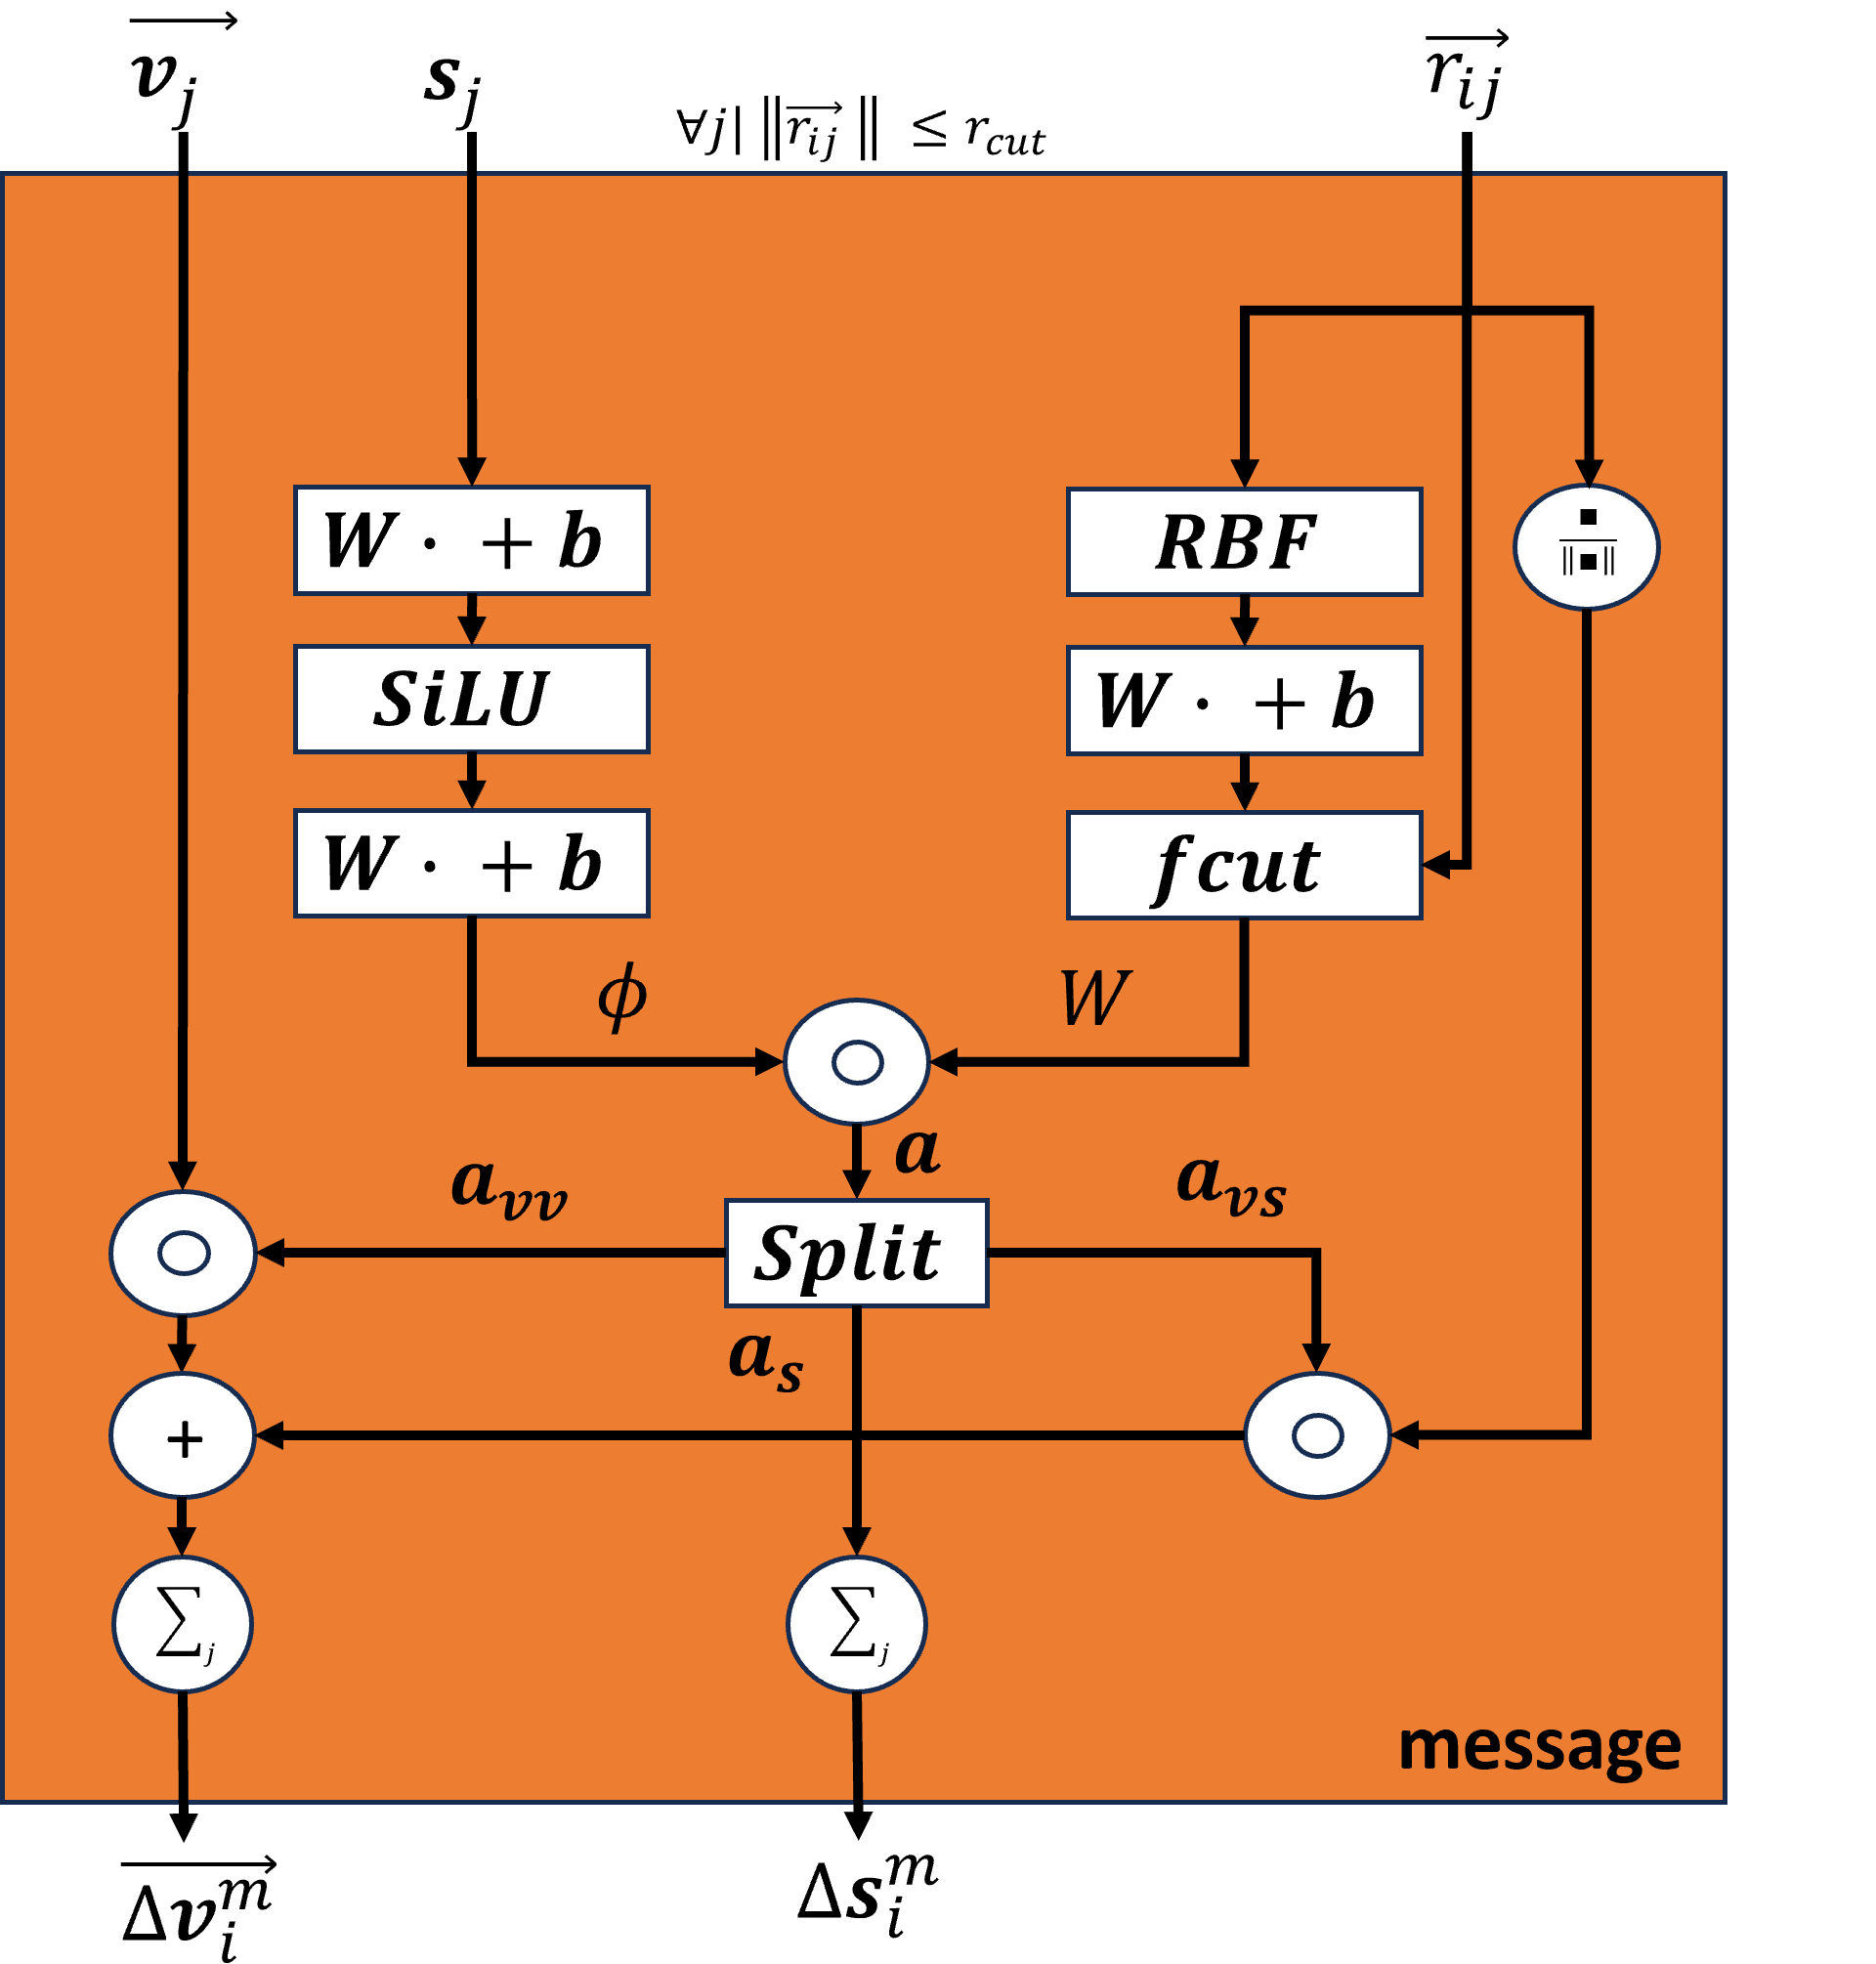
\includegraphics[width=250pt]{Images/Method/message_block.png}
\end{figure}






%#TODO fremhæv hvilke operationer som er invariante og equivariante, og hvorfor det er okay at nogen af operationerne ikke er equivariante
%#TODO papers til dette måske: Group equivariant convolutional networks, 2: Spherical CNNs, 3: n the generalization of equivariance and convolution in neural networks to the action of compact groups
%#TODO kom med en liste over ækvivariante operationer lidt ala som de har i PAINN



Equivariant representations of directions between nodes, have shown to be more expressive, at a similar computational cost.
This compared to rotationally invariant representations of either angular- or distance information
This effectively means a higher level of information can be maintained through the modelling phase, if the equivariance is
maintained.

Directional information is also expanded from the relative positions between edges $\vec{r}_{ij}$,
via the radial basis function (RBF)\cite{Atz2021}.The radial basis function outputs are chosen such that it is centered around twenty
points, $ C = \{1, 2, 3, \ldots, 20\}$. The function takes directional information $d = \lVert \vec{r}_{ij} \rVert$ and a cutoff
$r_{cut}$, and produces expansions following the formula below.

\begin{equation}\label{eq:rbf}
    \mathbf{RBF}(d) = \sum_{c \in C}\sin \left( \frac{c \pi}{r_{cut}} * d  \right) / d
\end{equation}
%#TODO Der skal ikke summes her, men laves 20 individuelle punkter for hver retning
%#TODO Hvad kig kildekoden til PAINN igennem for at se om RBF kommer før f_cut

The expansions provides a representation of similarity or dissimilarity, between the input relative position $\vec{r}_{ij}$,
and the chosen points $C$ \cite{rbf}. This information is further expanded by a neural network layer with a set of weights
biases, seen in equation \ref{eq:wandb}, before arriving at the cosine cutoff.

\begin{equation}\label{eq:wandb}
    y_{rbf} = \mathbf{w} \cdot \mathbf{RBF}(d) + \mathbf{b}
\end{equation}

The cosine-cutoff function is originally derived from \cite{Behler2011}
in the form of the equation below\ref{eq:coscutoff}.

\begin{equation}\label{eq:coscutoff}
    \begin{aligned}
        \mathbf{f}_{cut}(x) & =
        \begin{cases}
            0.5 \cdot \cos \left( \frac{\pi d}{r_{cut}} + 1  \right) & \text{if } d \leq r_{cut} \\
            0                                                        & \text{if } d > r_{cut}    \\
        \end{cases}
    \end{aligned}
\end{equation}

The cutoff function implemented in this project, utilized the equation below\ref{eq:coscutoffproject}:

\begin{equation}\label{eq:coscutoffproject}
    \begin{aligned}
        \mathbf{f}_{cut}(x) & =
        \begin{cases}
            0.5 \cdot \cos \left( \frac{\pi d}{r_{cut}} + 1  \right) \cdot y_{rbf} & \text{if } d \leq r_{cut} \\
            0                                                                      & \text{if } d > r_{cut}    \\
        \end{cases}
    \end{aligned}
\end{equation}

This alteration allows for the flow of information from both the radial basis expansions and the initial vector differences,
which from the process diagram in\cite{PAINN}, is not happening, although this is believed by the project to be the intention.
These three highlighted steps, the rbf, the set of weights and biases and the cosine cutoff,
constitute the rotationally invariant filter $\mathcal{W}_{s}$, proposed by \cite{Gasteiger2020},
and \cite{Behler2011}, and have been highlighted in this section, due to the difference in approaches from these propositions.

\subsection{Ensembles}

Ensembles is a technique for combining the predictive performance of individual modelling approaches
and to as an extension measuring total uncertainty in the model.
In the context of MPNNs, ensembles can be created by training multiple models with different initializations,
and combining their predictions.

Let $\mathbf{y}_i$ be the predicted binding energy for molecule $i$ by model $M_k$, where $i$ represents the molecule index and $k$
represents the model index. The ensemble prediction $\hat{\mathbf{y}}_i$ can be calculated as the mean of the individual
model predictions, as done in\cite{Tran2019}:

\begin{equation}\label{eq:mean-ensemble}
    \hat{\mathbf{y}}_i = \frac{1}{T} \sum_{k=1}^T \mathbf{y}_i^{(j)} = \hat{\mu_{i}}
\end{equation}

where $T$ is the number of models in the ensemble. This format of calculation weights the inputs from each model equally,
similarly to if it was a uniformly weighted mixture model as in \cite{Busk2021}.

To estimate the uncertainty in the ensemble predictions, we can calculate the variance of the individual model
predictions\cite{Tran2019}:
%#TODO giv en matematisk definition på en bin, måske baseret på kvantiler

\begin{equation}\label{eq:variance-ensemble}
    \text{Var}(\hat{\mathbf{y}}_i) = \frac{1}{T} \sum_{k=1}^T (\mathbf{y}_i^{(k)} - \hat{\mathbf{y}}_i)^2 = \hat{\sigma^{2}_{i}}
\end{equation}

%#TODO lav alt over her til et særskilt underafsnit, og alt under her som et andet afsnit

Finally as the foundation of estimating uncertainty in the ensemble predictions, we can estimate the expected normal calibration error.
This method relies on sorting predictions of targets, in $K$ equal sized bins, computing the predicted root mean variance\ref{eq:rmv}.

\begin{equation}\label{eq:rmv}
    RMV_{k} = ?
\end{equation}
%#TODO brug ligning 10 til at producere: kvadratroden af den gennemsnitlige varians indenfor en given bin.

Thereafter producing the empirical root mean squared error\ref{eq:rmse}:

\begin{equation}\label{eq:rmse}
    RMSE_{k} = \sqrt{\frac{1}{k} \sum_{k=1}^K \left( \mathbf{y}_i^{(k)} - \hat{\mathbf{y}}_i \right)^2}
\end{equation}

and finally utilizing the expression, following equation the equation in\cite{Busk2021}:

\begin{equation}\label{eq:calibration-error}
    ENCE = \frac{1}{k} \sum_{k=1}^K \frac{|RMV_{k} - RMSE_{k}|}{RMV_{k}}
\end{equation}
%#TODO Sum skal gå over 'i', hvor 'i' er alle værdier i en given bin

The approach of \cite{Busk2021} is based on models in an ensemble, outputting both a mean value and a variance metric, effectively
predicting both the target, and predicting its own uncertainty. This is not the case in this project, since the model solely predicts
the target.

\subsection{Model}\label{subsec:model}
%#TODO Flyt hele dette afsnit ned til theory section

The model architecture consists of two main components, namely the Message block, and the Update block as formerly introduced in the
the theory section \ref{eq:message_block}, and \ref{eq:update_block}.  The Message block is conceptually responsible
for the message passing between the nodes in the graph, allowing for the flow of information between the nodes.
This information is then summed up and stored in state variables in the form of a scalar and vector representation.
This summation is done in a residual manner, following the implementation of the PAINN architecture\cite{PAINN}. An equation
defining the residual calculation of the scalar-properties\ref{eq:residual_scalar} and vector-properties\ref{eq:residual_vector}
can be found below, as well as an illustration of the message block\ref{img:message_block}.

\begin{figure}[H]
    \caption{Message Block}
    \centering\label{img:message_block}
    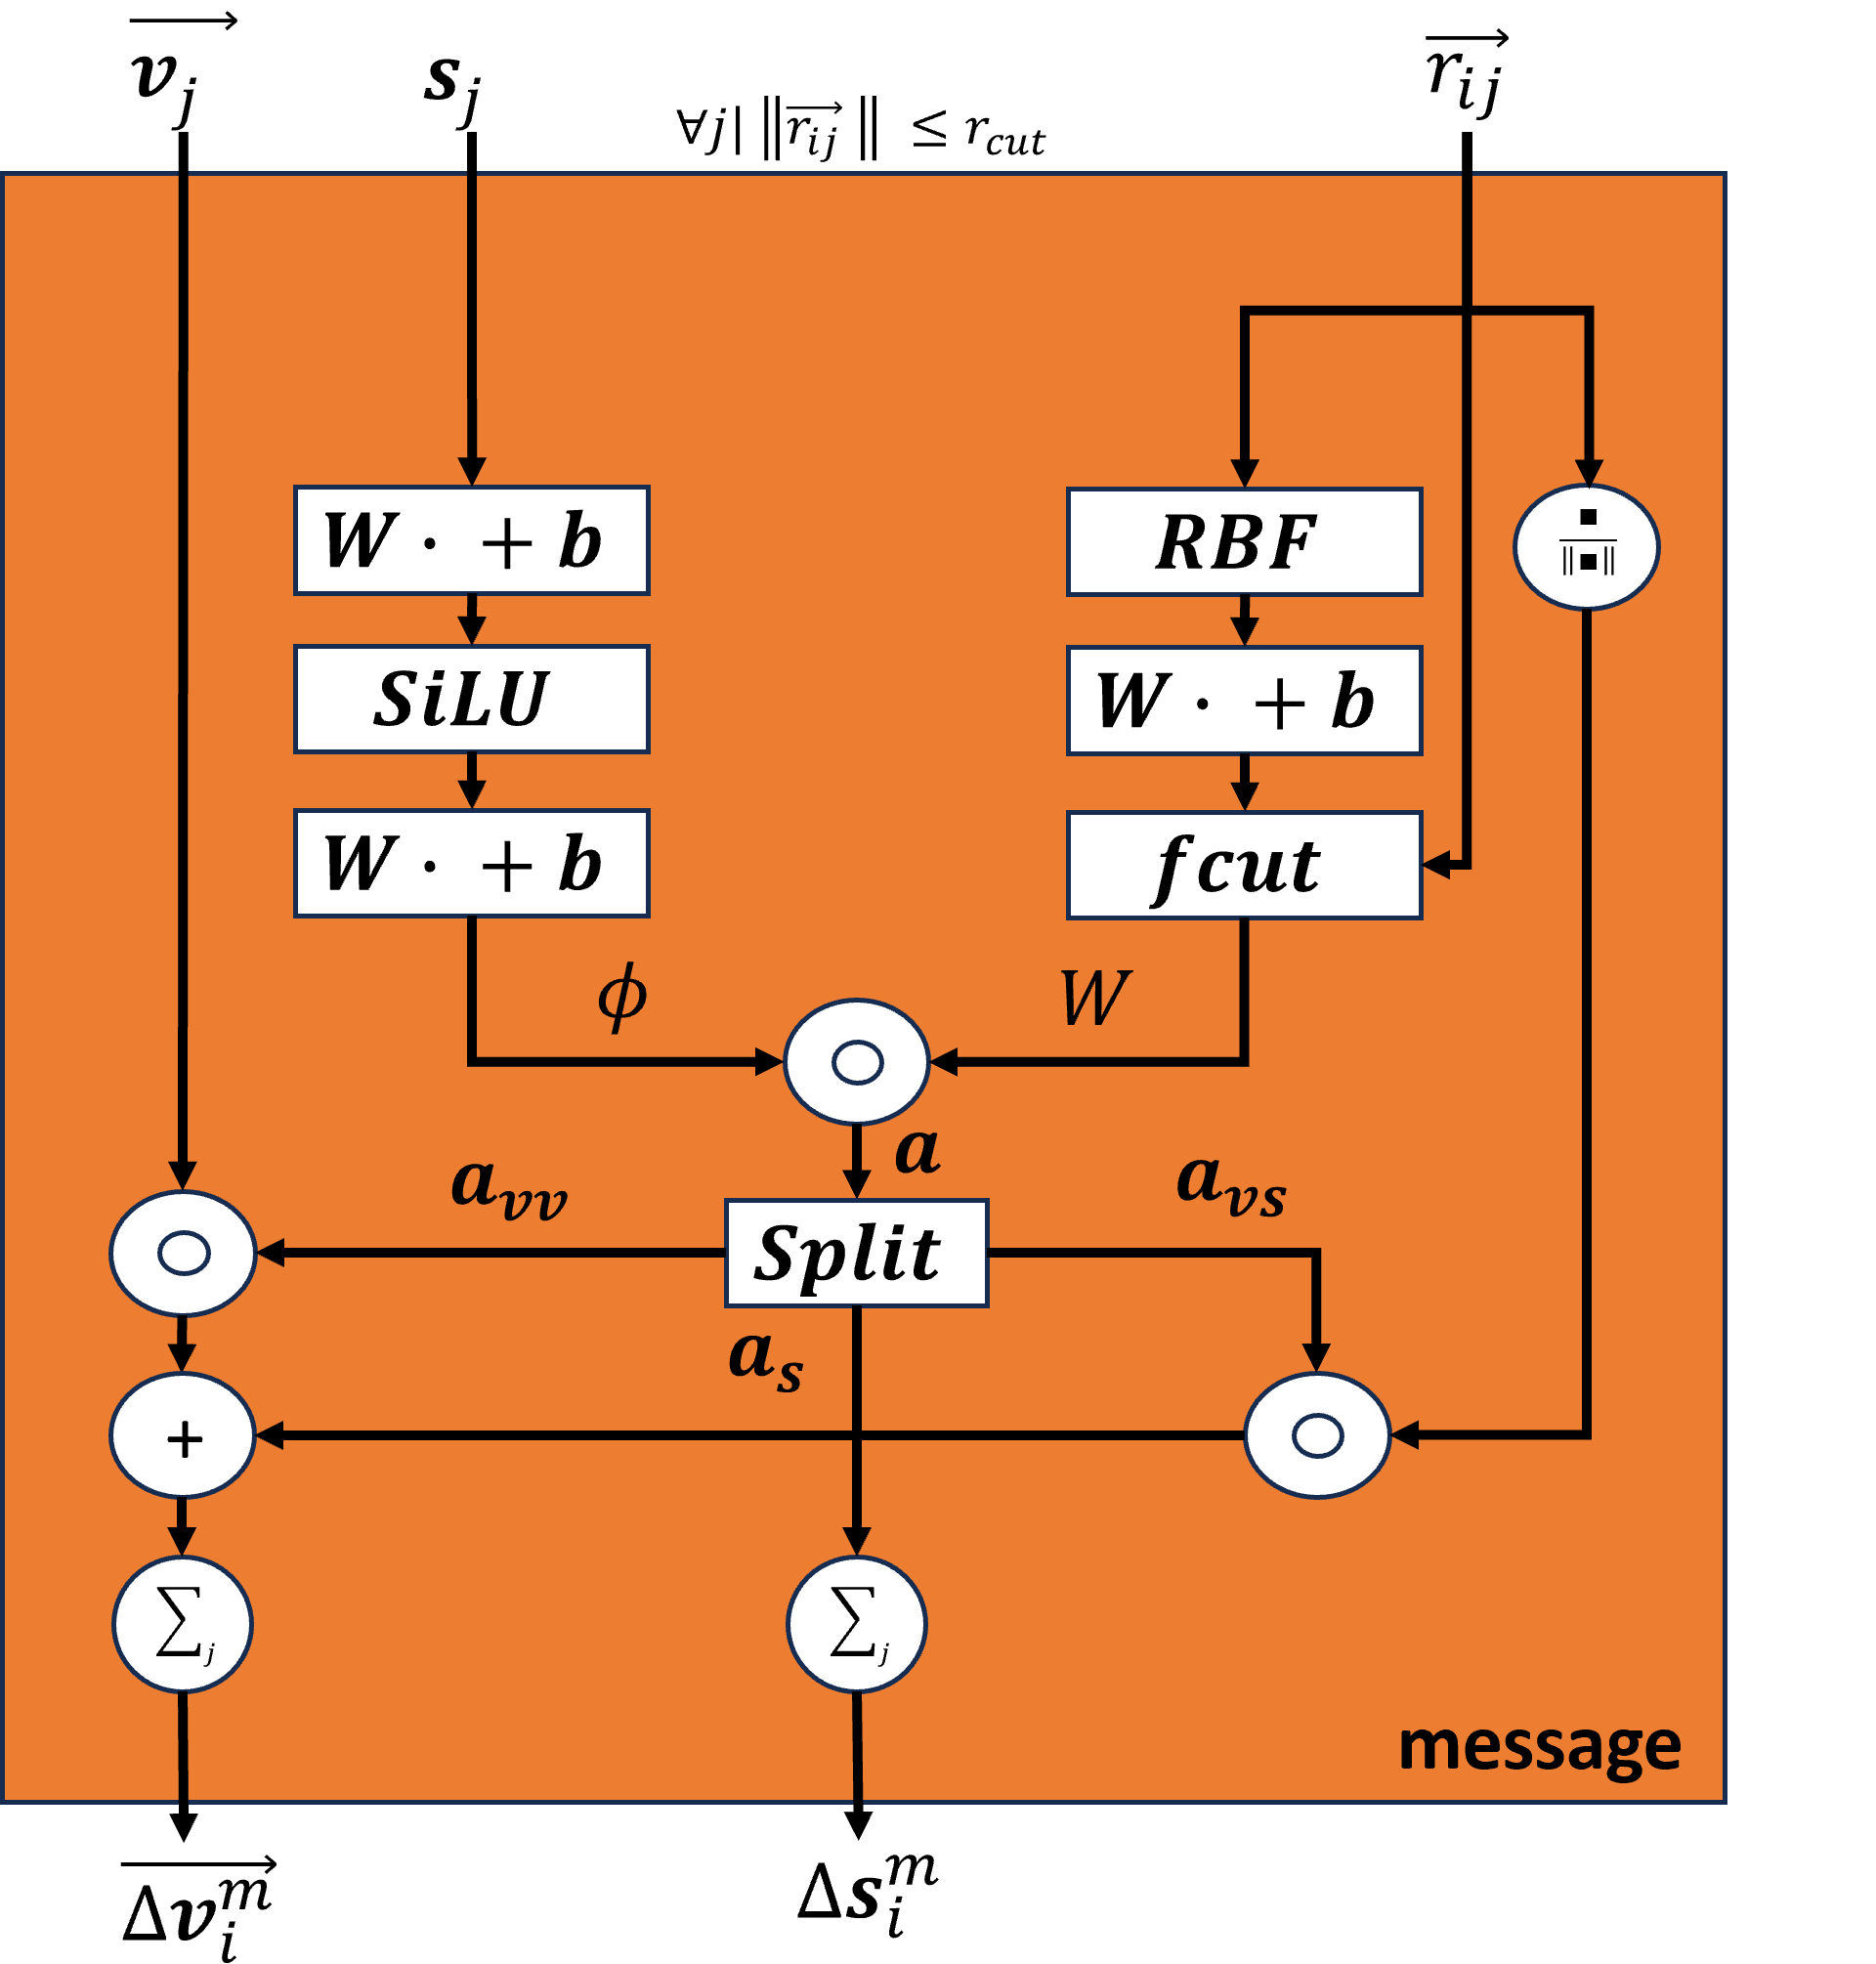
\includegraphics[width=250pt]{Images/Method/message_block.png}
\end{figure}

Worth noting about the figure, compared to the similar one in \cite{PAINN}, is the use of the \textit{r\_ij} vector, that also flow into
the 'fcut' function, as mentioned in \ref{subsec:modelling_task}. The model in this paper, does not highlight the dimension expansions
or collisions from network element to network element, due to the model parameters varying in size, as it is the scope of this project
to investigate similarities or dissimilarities in performance, with respect to the PAINN architecture and dissimilar state representation
sizes. both sizes $\phi$ and $\mathcal{W}$ are chosen sub-architectures based on the PAINN architecture from\cite{PAINN}. The image
also contains hints of the $\mathbf{a}$-tensor, which is a product of the $\phi$ and $\mathcal{W}$ tensors, and not highlighted in \cite{PAINN}.

The residual values produced in the message block, then used in the update block, in order to update the node states,
based on the summation over neighbouring states.
This structure is also heavily inspired by the PAINN architecture\cite{PAINN}. The below equations represent the residual updates
on both the scalar- \ref{eq:residual_scalar_update} and the vector- \ref{eq:residual_vector_update} properties. Below is also
a figure representing the update block\ref{img:update_block}.


\begin{figure}[H]
    \caption{Update block}
    \centering\label{img:update_block}
    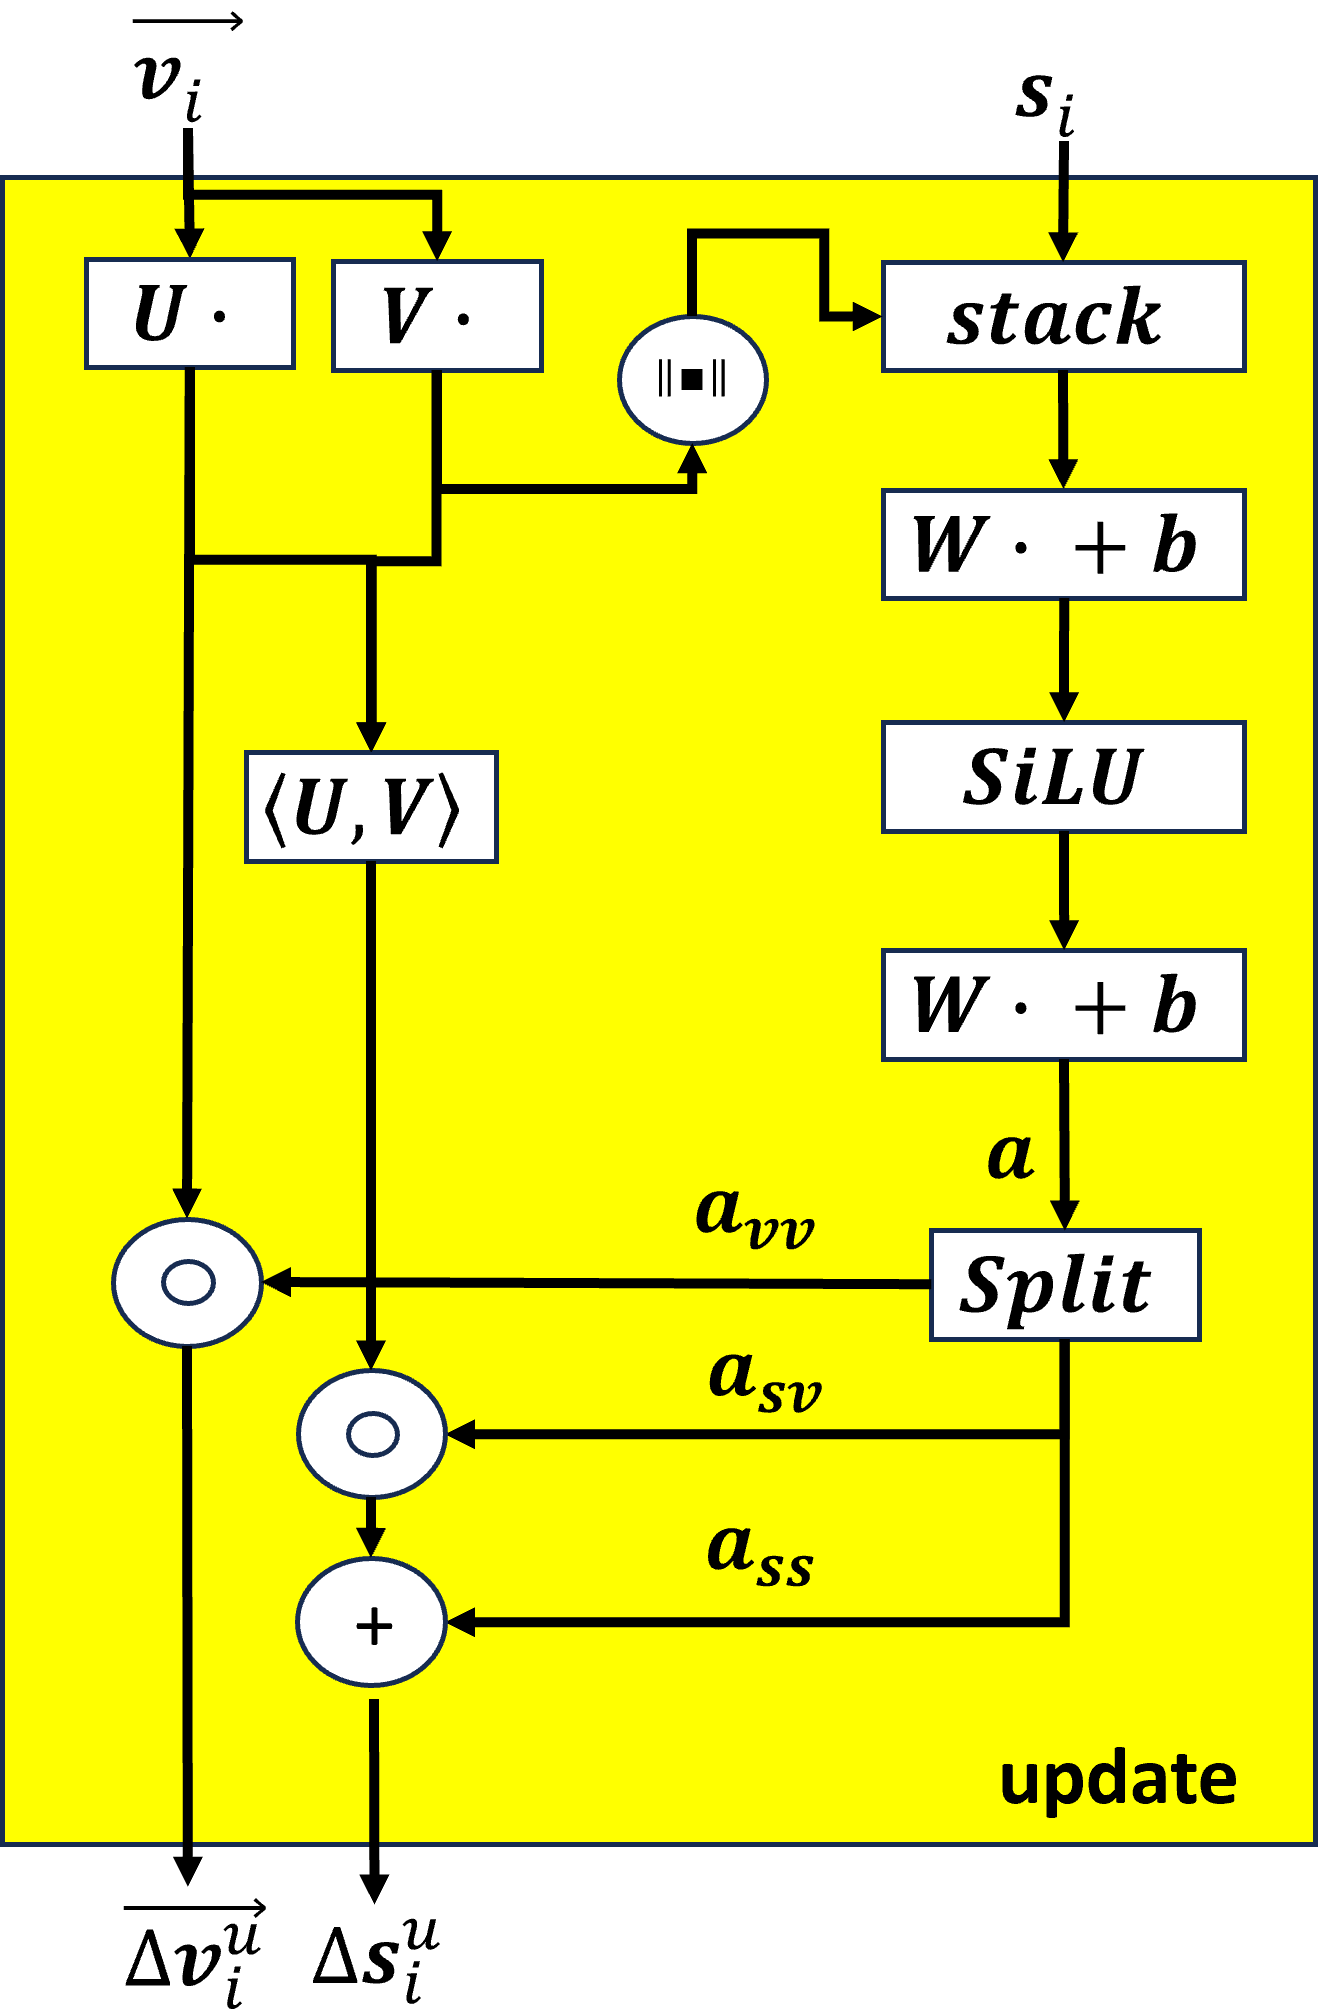
\includegraphics[width=250pt]{Images/Method/update_block.png}
\end{figure}

Worth noting about the above figure \ref{img:update_block}, is that the indexes of the scalar and vector representations,
have been altered, compared to \cite{PAINN}. This comes down to the project evaluating the indexing of the scalar and vector
representations, in the paper, were faulty, and did not represent the PAINN architecture as described in prior sections of the
paper.

The blocks are stacked in coupled sequences of five full rounds, like the illustration below highlights\ref{img:MPNN_arc}, a corresponsding model can be found
in \cite{PAINN}. The illustration shows an architecture comprised of three sets of message- and update-blocks, the implementation in this project utilized
five sets. The model representation property $\vec{v_i^{0}}$ is initialized to the zero vector, and the scalar property $S_{i}^{0}$
is initialized to a random embedding on atom level, for each node in the graph.


\begin{figure}[H]
    \caption{MPNN Full Architecture}
    \centering\label{img:MPNN_arc}
    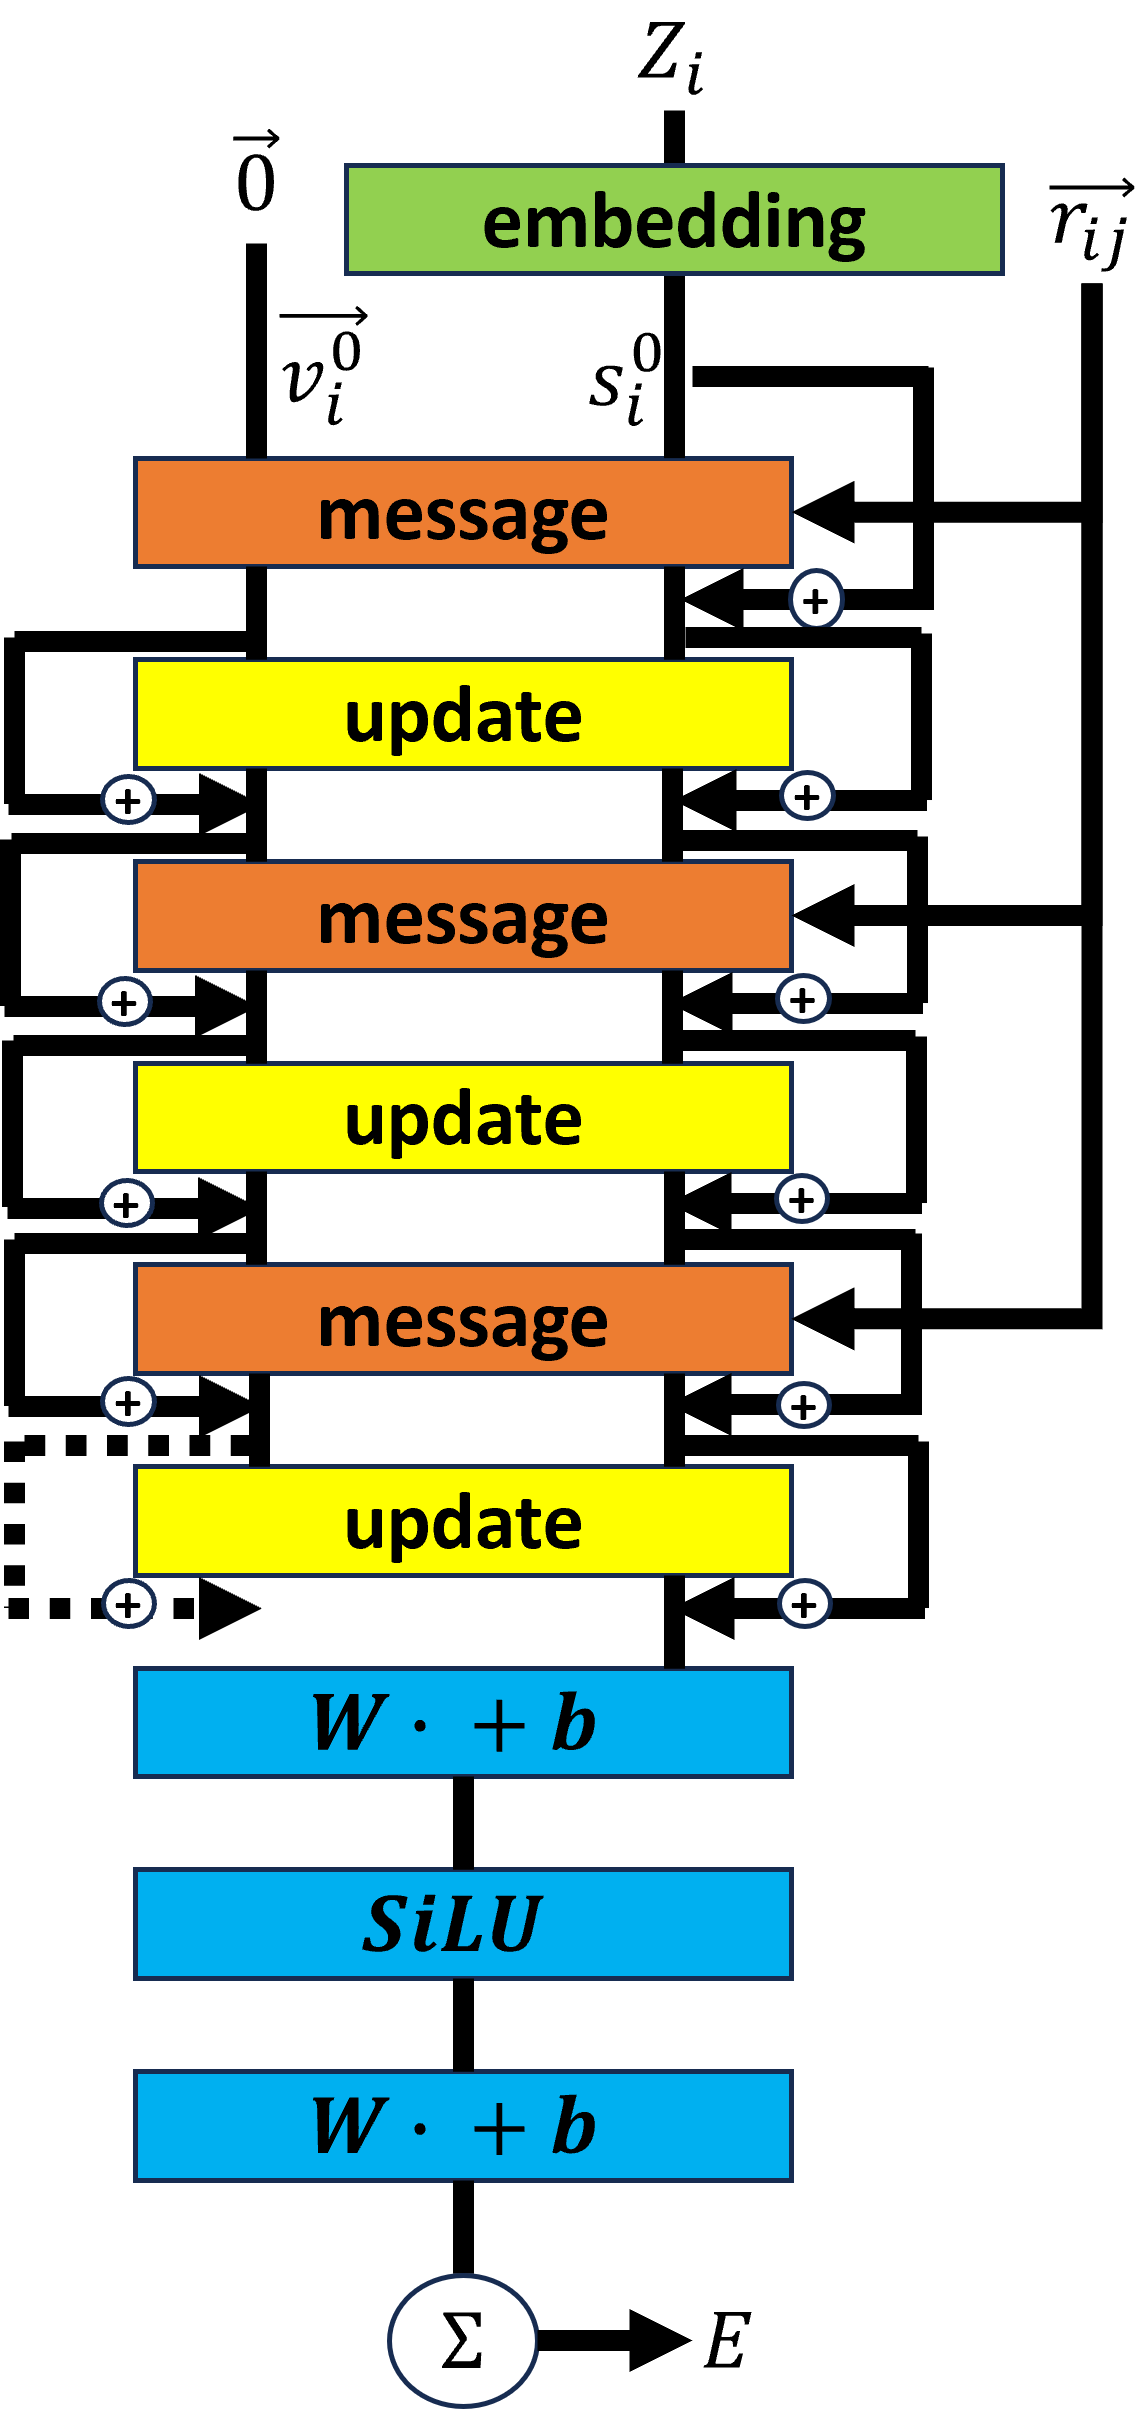
\includegraphics[width=200pt]{Images/Method/MPNN_arc.png}
\end{figure}


\newpage